%% Submissions for peer-review must enable line-numbering 
%% using the lineno option in the \documentclass command.
%%
%% Preprints and camera-ready submissions do not need 
%% line numbers, and should have this option removed.
%%
%% Please note that the line numbering option requires
%% version 1.1 or newer of the wlpeerj.cls file, and
%% the corresponding author info requires v1.2

\documentclass[fleqn,10pt,lineno]{wlpeerj} % for journal submissions
% \documentclass[fleqn,10pt]{wlpeerj} % for preprint submissions

%\usepackage{hyperref}
\usepackage{setspace}
% \usepackage{gensymb}
% \usepackage{xcolor} % added by NJG for edits

\title{Expanded view of the ecological genomics of ant responses to
  climate change}

\author[1]{Matthew K. Lau}
\author[1]{Aaron M. Ellison}
\author[2,3]{Andrew Nguyen}
\author[4,5]{Clint Penick}
\author[6]{Bernice DeMarco}
\author[2]{Nicholas J. Gotelli}
\author[7]{Nathan J. Sanders}
\author[4]{Robert Dunn}
\author[2]{Sara Helms Cahan}

\affil[1]{Harvard Forest, Harvard University, Petersham, MA, USA}
\affil[2]{Department of Biology, University of Vermont, Burlington,
  VT, USA}
\affil[3]{Department of Entomology and Nematology, University of
  Florida, Gainesville, FL, USA}
\affil[4]{Department of Applied Ecology, North Carolina State
  University, Raleigh, NC, USA}
\affil[5]{The Biomimicry Center, Arizona State University, Tempe, AZ, USA}
\affil[6]{Smithsonian Institution, Washington, DC, USA}
\affil[7]{Environmental Program, Rubenstein School of Environment and Natural Resources, University of Vermont, Burlington, VT, USA}

\corrauthor[]{Matthew K. Lau}{matthewklau@fas.harvard.edu}

%% \keywords{genomics, biogeography, climate change, ants, Formcicidae}
\begin{abstract}

Ecological genomics provides a window into potential responses of
organisms to environmental change. Given the abundance, broad
distribution and diversity of roles that ants play in many ecosystems,
they are an ideal group to serve as ecosystem indicators of climatic
change. At present, only a few whole-genome sequences of ants are
available (19 of $>$ 16,000 species), mostly from tropical and
sub-tropical regions.  To address this, we sequenced the genomes of
seven whole colonies of six species from the genus
\textit{Aphaenogaster}:  \textit{A. ashmeadi}, \textit{A. floridana},
\textit{A. fulva}, \textit{A. miamiana}, \textit{A. picea}, and
\textit{A. rudis}. The geographic ranges of these species collectively
span eastern North America from southern Florida to southern Canada,
which comprises a latitudinal gradient in which many climatic
variables are changing rapidly. For the six genomes, we assembled an
average of 271,039 contigs into 47,337 scaffolds. The mean genome size
was 270 Mb, which was comparable to that of other sequenced ant
genomes (212.83 to 396.03 Mb).  Looking across all currently sequenced
ant genomes, we found support for a relationship between biogeographic
variables and genome similarity and size. The strongest correlations
were between genomic similarity and two main groups of climate
variables relating to cold temperatures and precipitation. These
results point to climate as a mechanism leading to genomic differences
in ants and provide a point of departure for future work that explores
the responses of ants to climatic change at the interface of ecology
and evolution.

\end{abstract}



\begin{document}

\flushbottom
\maketitle
\thispagestyle{empty}

%% \subsection*{About PeerJ}

%% PeerJ is an award-winning open access publisher covering the
%% biological and medical sciences.  PeerJ provides authors with three
%% publication venues: \textit{PeerJ} and \textit{PeerJ Computer Science}
%% (peer-reviewed academic journals) and \textit{PeerJ PrePrints} (a
%% 'pre-print server'). See https://peerj.com/about/publications/ for
%% more information.

%% The PeerJ model allows an author to publish articles in their
%% peer-reviewed journal via the purchase of a lifetime Publication
%% Plan. Prices start from just \$99 (a one-off payment) which entitles
%% an author to the lifetime ability to publish 1 article per year for
%% free. Publication in PeerJ PrePrints is entirely free.

%% If you have a question, please use the help menu in the top right of
%% the screen to get in touch. When your article or pre-print is
%% complete, use the "Submit to PeerJ" button in the topbar to send your
%% files to PeerJ.

\abstract

\doublespacing

\section*{Introduction}

Understanding how terrestrial ecosystems will respond to ongoing
shifts in climatic variables, such as temperature and precipitation,
will improve our ability to manage communities and mitigate impacts of
climatic change. The mean global temperature is currently on track to
meet or exceed that predicted by the most extreme forecasting models
\citep{Brown2017}. Climatic change is also pushing local conditions
outside the boundaries of historic ranges, potentially leading to
combinations of species or entire ecosystems that have no contemporary
analogs that are challenging to predict accurately
\citep{Burrows2014}. Also, as climate driven impacts on evolutionary
responses are likely to occur over contemporary time-scales, there is
a need for a comprehensive study of the genetic basis of species'
climate responses to understand and potentially predict the responses
of ecosystems to climate change \citep{Parmesan2006a, Diamond2018}.


The biodiversity of most terrestrial systems is great enough to be
intractable to study in its entirety. To deal with this, researchers
often study `indicator' species whose responses to environmental
change are broadly representative of a much wider range of taxa
\citep{Siddig2016}. Ants (Formicidae) are widely used as indicator
taxa \citep{Agosti2000} because they play key roles in community
dynamics and ecosystem processes, including key interactions, such as
seed dispersal and the movement of soil via colony construction
\citep{DelToro2012}. Ants are also responsive to changes in
temperature and other climatic variables via individual responses,
changes in social structure and commnity assembly \citep{Spicer2017,
  Diamond2017, Diamond2018}. Seed dispersers in particular are likely
to to respond to climate change, as there is evidence demonstrating
that climate change may have strong negative impacts on female
individuals of dioecious plant species \citep{Hultine2016}. This is
leading to decreased abundance of female individuals and reductions in
seed production with potentially cascading impacts on associates,
including seed dispersers such as myrmecochorus ants.

In eastern North America and temperate Asia, species of the genus
\textit{Aphaenogaster} are abundant understory ants that play key
roles in the dispersal of seeds. Previous studies have shown
\textit{Aphaenogaster} species respond to climatic change, and the
response of these species to climatic change appears to depend both on
the species being studied and on the geographic region in which
climatic change occurs. \cite{Warren2013} found that shifts in the
distribution of two \textit{Aphaenogaster} species, \textit{A. rudis}
and \textit{A. picea}, were determined by minimum
temperatures. \cite{Diamond2016} reported that the rate of
colonization and occupancy of nests by \textit{Aphaenogaster} species
in a five-year experimental warming study \citep{Pelini2014} declined
with temperature in the warm, southern study site (Duke Forest, NC,
USA) but not in the cooler, northern study site (Harvard Forest, MA,
USA).

In addition to ants serving as indicators of ecological impacts of
climatic change, ant genetics may provide insights into the potential
responses of ant assemblages. One study has found that ant colony
development is experiencing climate related selection pressure
\citep{Penick2017} and previous work has demonstrated that
phylogenetics is a factor determining the response of ant species to
climatic change \citep{Diamond2012a}. A comparative study of the
southern, more warm-adapted, \textit{A. carolinensis} displayed a
greater reduction in the regulation of suites of genes in response to
experimental warming than did the cold-adapted \textit{A. picea}
\citep{Stanton-Geddes}, suggesting a genetic component to temperature
response. At the macroevolutionary scale, there is evidence for
temporal synchrony in major transitions of terrestrial plant
communities and the diversification of ant lineages. \cite{Moreau2006}
showed that the evolution of \textit{Aphaenogaster} was coincident
with the shift from gymnosperm to angiosperm dominated forests in the
early to middle Paleogene.

Although these and other studies (see \cite{Nygaard2015}) support the
perspective that a more complete knowledge of ant genetics will
increase our understanding of ant responses to environmental change
\citep{Boomsma2017}, at present relatively few ant species have been
sequenced ---20 in total, of which 19 are currently available in the
NCBI Genome Database (accessed April 1 2018, see
Table~\ref{tab:ncbi_ants}). Of these, most are from tropical and
subtropical assemblages, and all but five represent unique genera (the
exceptions being two species of \textit{Atta} and three of
\textit{Trachymyrmex} (Fig~\ref{fig:ant_world_usa}). No species of
\textit{Aphaenogaster} have yet been sequenced.

\begin{figure}[ht]
\includegraphics[width = 0.9\textwidth]{gaga_world.pdf}
\caption{Number of whole-genome sequences available in NCBI by country
  (accessed April 2018).}
\label{fig:ant_world_usa}
\end{figure}

% latex table generated in R 3.4.2 by xtable 1.8-2 package
% Fri Dec 15 14:16:56 2017
\begin{table}[ht]
\centering
\begin{tabular}{lll}
  \hline
Ant Species & BioProject Accession & BioSample Accession \\ 
  \hline
Acromyrmex echinatior & PRJNA62733 & SAMN02953789 \\ 
  Atta cephalotes & PRJNA48091 & SAMN02953774 \\ 
  Atta colombica & PRJNA343260 & SAMN03982875 \\ 
  Camponotus floridanus & PRJNA50201 & SAMN02953777 \\ 
  Cyphomyrmex costatus & PRJNA343963 & SAMN03982885 \\ 
  Dinoponera quadriceps & PRJNA301625 & SAMN02869781 \\ 
  Harpegnathos saltator & PRJNA50203 & SAMN00016742 \\ 
  Lasius niger & PRJNA269328 & SAMN03253098 \\ 
  Linepithema humile & PRJNA45799 & SAMN02767796 \\ 
  Monomorium pharaonis & PRJDB3164 & SAMD00020277 \\ 
  Ooceraea biroi & PRJNA275884 & SAMN02428046 \\ 
  Pogonomyrmex barbatus & PRJNA45797 & SAMN02953770 \\ 
  Pseudomyrmex gracilis & PRJNA377720 & SAMN03219222 \\ 
  Solenopsis invicta & PRJNA49629 & SAMN02953778 \\ 
  Trachymyrmex cornetzi & PRJNA343972 & SAMN03982882 \\ 
  Trachymyrmex septentrionalis & PRJNA343973 & SAMN03982881 \\ 
  Trachymyrmex zeteki & PRJNA343251 & SAMN03982884 \\ 
  Vollenhovia emeryi & PRJDB3517 & SAMD00026325 \\ 
  Wasmannia auropunctata & PRJDB3443 & SAMD00024919 \\ 
   \hline
\end{tabular}
\caption{NCBI genome database accession information for the previously sequenced ant genomes.} 
\end{table}


To increase the number of genomes of temperate-zone ant species for
other genetic studies (e.g. short-read and target sequences or
transcriptomics), we sequenced the entire genomes of six
\textit{Aphaenogaster} species from eastern north america:
\textit{A. ashmeadi}, \textit{A. floridana}, \textit{A. fulva},
\textit{A. miamiana}, \textit{A. picea} and \textit{A. rudis}. These
species were collected from across a broad biogeographic gradient
spanning 10 degrees of longitude and 12 degrees of latitude. With the
these new whole-genome sequences and the full set of publicly
available ant genomes (NCBI), we test two hypotheses about the factors
influencing the distribution of ant genomes. First, to test the
hypothesis that climate variables shape the distribution of ant
genomes, we explored the correlation between spatial and multi-decadal
climate variables. If evolutionary dynamics in ants have been
influenced by environmental conditions, then ant genomes from more
similar conditions will have more similar genomes. Second, as previous
work has demonstrated patterns in the evolutionary dynamics of ant
genome size \citep{Tsutsui2008a} and empirical studies of have
reported biogeographic patterns in genome size in other arthropod
taxa, e.g. Crustacea \citep{Hultgren2018}, we also tested the
hypothesis that ant genome size exhibits biogeographic
patterns. Because previous studies of ant genome size suggest that
selection can act on genome size and that genome size is influenced by
phylogeny \citep{Tsutsui2008a}, we predicted that genome size
similarity would also be positively correlated with environmental
similarity.  We present the results of this sequencing effort and use
of the entire set of ant genomes to test the hypotheses of
biogeographic patterns in ant genome sequence similarity and size.


\section*{Results}

\subsection*{Whole-genome Sequencing}

Entire colonies of the six \textit{Aphaenogaster} species were
collected by A. Nguyen and C. Penick from field sites in eastern North
America (Fig~\ref{fig:sampling}). Ants were identified to species and
specimens from these colonies are preserved at the University of
Vermont, North Carolina State University and the Museum of Comparative
Zoology at Harvard University. Individuals from each colony were
isolated from nest material and debris, weighed, placed in 50 ml
Falcon centrifuge tubes and immediately flash frozen in a
$-80^{\circ}$ C freezer. Colony weights were: 794.0 mg
(\textit{A. ashmeadi}), 652.0 mg (\textit{A. floridana}), 520.0 mg
(\textit{A. fulva}), 749.0 mg (\textit{A. picea}), 862.0 mg
(\textit{A. miamiana}), 280.0 mg (\textit{A. rudis} 1) and 236.0 mg
(\textit{A. rudis} 2).

\begin{figure}[ht]
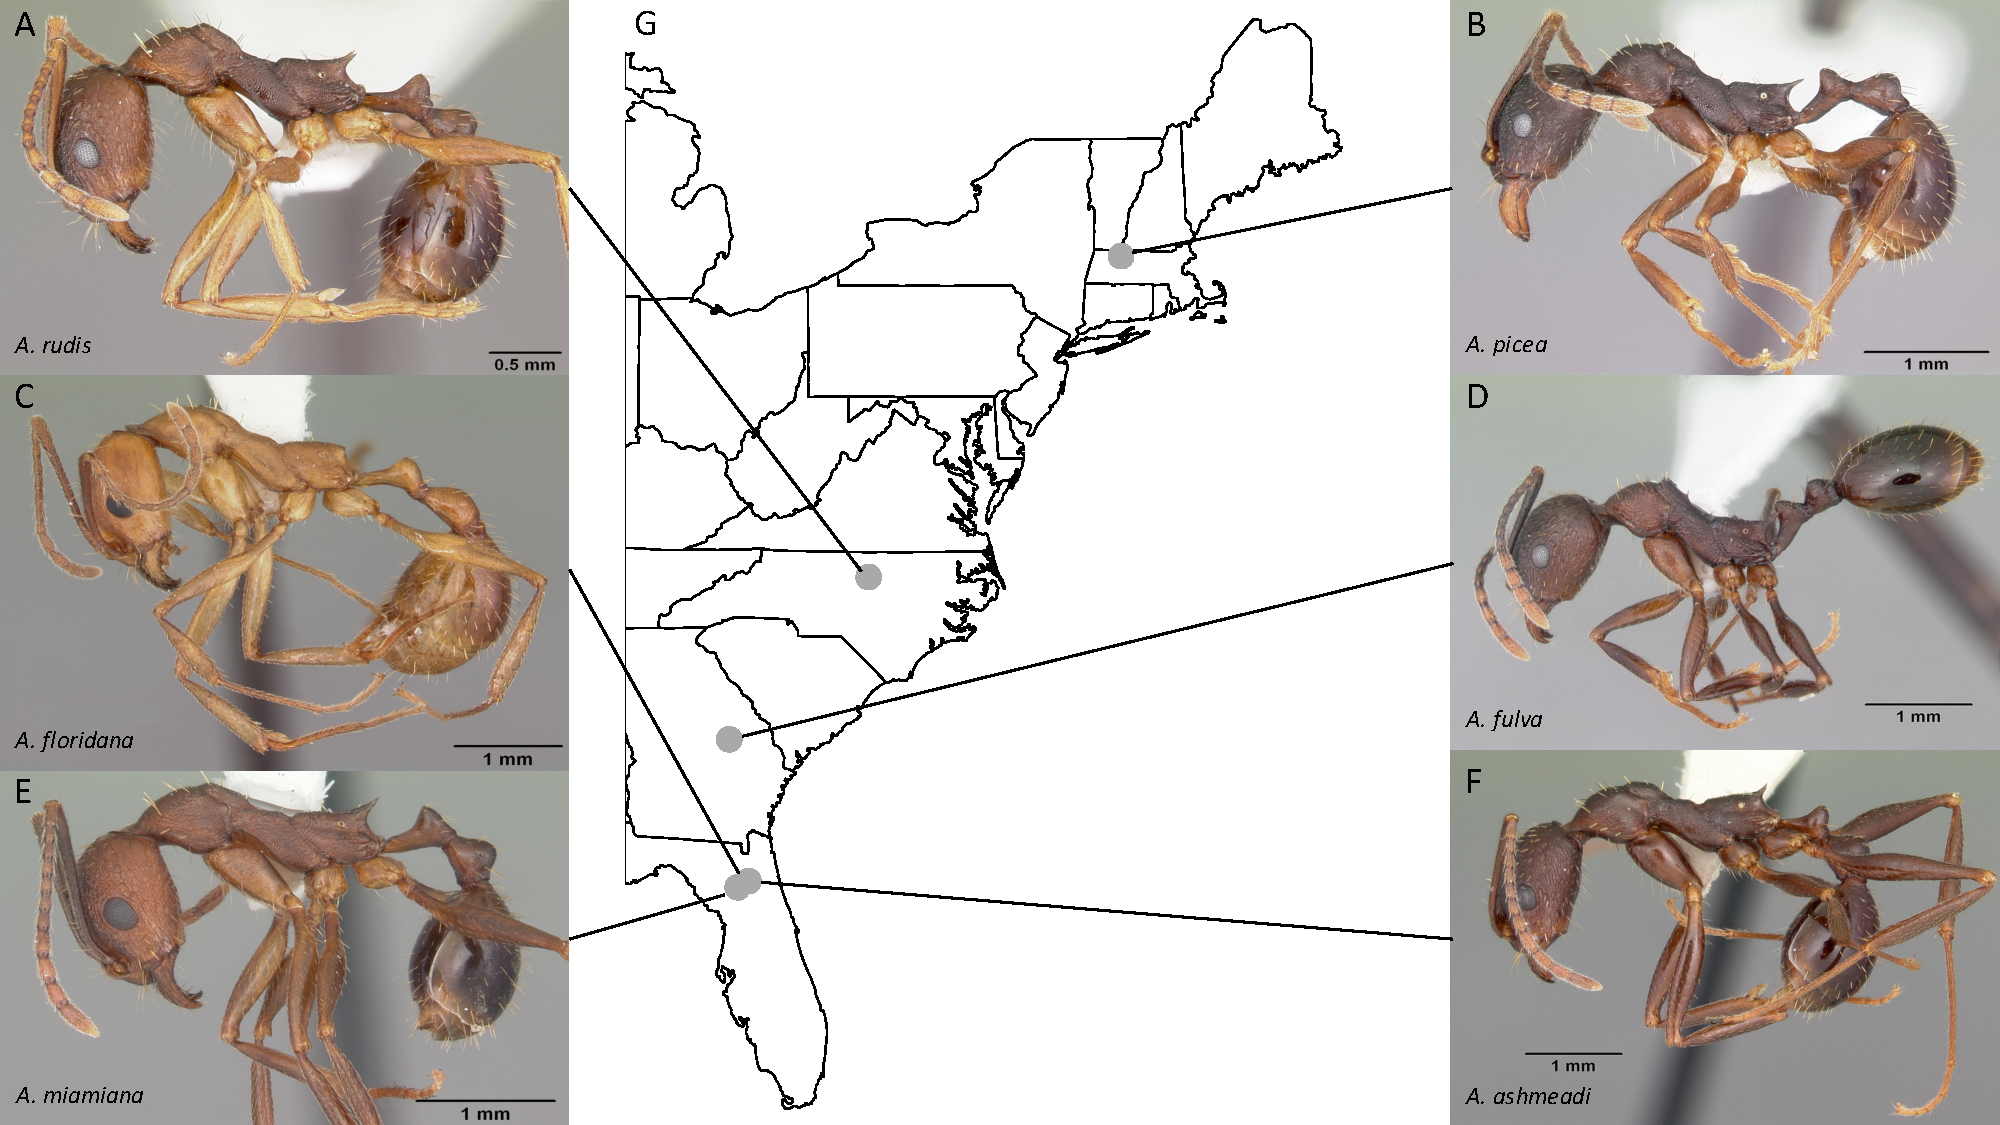
\includegraphics[width = 0.9\textwidth]{map_apg.pdf}
\caption{We sampled seven colonies representing six species of
  \textit{Aphaenogaster} from across eastern North America (see
  Table~\ref{tab:climate}). All photos by April Noble (available from
  http://www.antweb.org).}
\label{fig:sampling}
\end{figure}

DNA was then extracted from each colony using methods developed
previously for genomic sequencing of whole colonies of mosquitos
(\textit{Anophales} spp.)  \citep{Neafsey2010} and sequenced using an
illumina hiseq 2500 at the broad institute (Cambridge, MA, USA). a
combination of fragment and jump sequences were used to generate
higher quality, long sequence reads. Raw sequences were processed to
remove chimeric and contaminant sequences, screened for contaminants
by blast searches to identify sequences with likely matches to
non-target species (primarily \textit{Wolbachia} and
\textit{Mycoplasma}), and assembled using ALLPATHS-LG (version r48559)
\citep{Gnerre2011}. Additional assembly processing using PILON
(version 1.13) \citep{Walker2014} was applied to reduce base-call
errors and gaps in coverage. On average, across all seven genomes,
PILON reduced coverage gaps by 3.1\% or 3.9 mb. GAEMR
(http://www.broadinstitute.org/software/gaemr/) software produced
summary statistics of the final assembled genomes.

% latex table generated in R 3.4.2 by xtable 1.8-2 package
% Tue Mar 20 17:26:28 2018
\begin{table}[ht]
\centering
\begin{tabular}{rrrrrr}
  \hline
 & Lat & Lon & Tmin (C) & Tmax (C) & Precip (mm) \\ 
  \hline
{\emph{Aphaenogaster ashmeadi}} & 29.79 & -82.03 & 6.11 & 33.13 & 1290.40 \\ 
  {\emph{Aphaenogaster floridana}} & 29.79 & -82.03 & 6.11 & 33.13 & 1290.40 \\ 
  {\emph{Aphaenogaster fulva}} & 32.69 & -82.51 & 1.83 & 33.81 & 1156.81 \\ 
  {\emph{Aphaenogaster miamiana}} & 29.66 & -82.30 & 5.87 & 32.75 & 1254.72 \\ 
  {\emph{Aphaenogaster picea}} & 42.60 & -72.58 & -11.11 & 28.12 & 1199.06 \\ 
  {\emph{Aphaenogaster rudis1}} & 36.02 & -78.98 & -1.82 & 31.60 & 1168.41 \\ 
  {\emph{Aphaenogaster rudis2}} & 36.02 & -78.98 & -1.82 & 31.60 & 1168.41 \\ 
   \hline
\end{tabular}
\caption{Climate variables for colony sample sites. Climate are 30 year normal values (1976-2016) for January minimum temperature (Tmin), July maximum temperature (Tmax) and total precipitation (Precip).} 
\label{tab:climate}
\end{table}


\subsection*{Genome Quality and Composition}

DNA extractions yielded substantial amounts of high quality DNA with
concentrations and quality scores ranging from 3.45\textendash5.39
ng$\mu$L$^{-1}$ and 4.05\textendash4.27 ng$\mu$L$^{-1}$,
respectively. All genome assemblies displayed good coverage, with an
average of 70\% of fragments mapped (Table
\ref{tab:assemblystats}). Across all species, the length of the
shortest contig at 50\% of the genome (i.e. N50) was 18,864 bases;
average assembly GC content was 38.18\%; and average genome size was
471 Mb.  using a BLAST search of the contigs and the NCBI sequence
database, we found that 38.98\% and 22.04\% of the top hits were
``ant'' and \textit{Aphaenogaster}, respectively. the
\textit{Aphaenogaster} genomes compared well with other ant genome
sequences. the sizes of the \textit{Aphaenogaster} genomes were within
the range of other ant genomes based on size from both flow-cell
cytometry \citep{Tsutsui2008a} and the previously sequenced ant
genomes available in NCBI (Fig~\ref{fig:ncbi_compare}). The scaffolds
were within the range recommended for gene coverage based on
\citet{Efron2007}.


%%% assembly statistics table. 
\input{assembly_stats}


\begin{figure}[ht]
\includegraphics[width = 0.90 \textwidth]{ncbi_gaga_compare.pdf} 
\caption{the size of sequenced \textit{Aphaenogaster} genomes were
  within the size range of previously published observed or estimated
  genomes of ants. frequency distribution of previously published
  genome size estimates using flow cytometry from \cite{Tsutsui2008a}
  and those available via NCBI (accessed April 2018). Vertical lines
  identify the sizes of the \textit{Aphaenogaster} assemblies (see
  Table~\ref{tab:assemblystats}).}
\label{fig:ncbi_compare}
\end{figure}

We observed patterns in genomic composition that generally were
consistent with expectations based on phylogenetic relatedness. After
detecting and masking repeat regions in the \emph{Aphaenogaster}
genomes using \textit{Repeatmasker} (version 4.0.5 Institute for
Systems Biology), we applied MASH distance \citep{Ondov2016} to
measure pairwise dissimilarity of genomic sequences. The MASH method
extends a data compression and dimensionality-reduction algorithm to
generate estimates of sequence similarity with low computational
overhead. Briefly, the pairs of genomic sequences were pre-processed
into sets of k-mers of size 21 with the size of the non-redundant
hashes retained set to 1,000. These settings have been demonstrated to
provide good representation of genomic similarity with minimal
computational costs \citep{Ondov2016}. These sets were then used to
estimate the Jaccard similarity coefficient (the ratio of shared
k-mers to total k-mers) of subsampled k-mer pairs of genomes. This
unbiased estimate of the Jaccard similarity ($J$) was then used to
calculate the dissimilarity of the two genomes ($D$) as $D = 1 -
J$. All Jaccard similarity estimates had \textit{p}-values less than
$10^{-14}$, which is below the recommended $10^{-3}$ probability of
observing values of $J$ due to chance.

Using the MASH genomic distances, we observed patterns of genomic
similarity in-line with expectations from established ant
phylogenetics. Sequences formed groups that corresponded with
subfamily (Fig~\ref{fig:all_heat}). \textit{Aphaenogaster} clustered
with other genera from the \textit{Myrmicinae} and, in general,
subfamily level clustering tended to follow previously observed
patterns of subfamily relatedness \citep{Bolton2006, Moreau2006,
  Ward2014}.  The \emph{Aphaenogaster} sequences formed a single
cluster containing only \emph{Aphaenogaster} species and displayed
intra-generic levels of genomic variance comparable to other genera
(e.g., \textit{Trachymyrmex} spp.). The separation of the two
\textit{A. rudis} species was initially surprising, as these two
samples were collected at the same site (Duke Forest, NC USA) and were
identified as the same species based on their morphological
characteristics \citep{Ellison2012, Demarco2016}. However, two recent
studies of targeted gene regions have demonstrated the polyphyletic
nature of \textit{Aphaenogaster rudis}.  One study of the evolution of
the subfamily \textit{Myrmicinae} observed that the genus as a whole
could be split into at least four different lineages
\citep{Ward2015}. Another, more detailed study of the genus in North
America found that multiple individuals of \textit{A. rudis} separated
out into distinct groupings, each with other species, specifically,
individuals of \textit{A. rudis} from North Carolina (USA) were
observed to form distinct clusters with individuals of
\textit{A. carolinensis}, \textit{A. miamiana},
\textit{A. lamellidens} and \textit{A. texana} \citep{Demarco2016}.


\begin{figure}[ht]
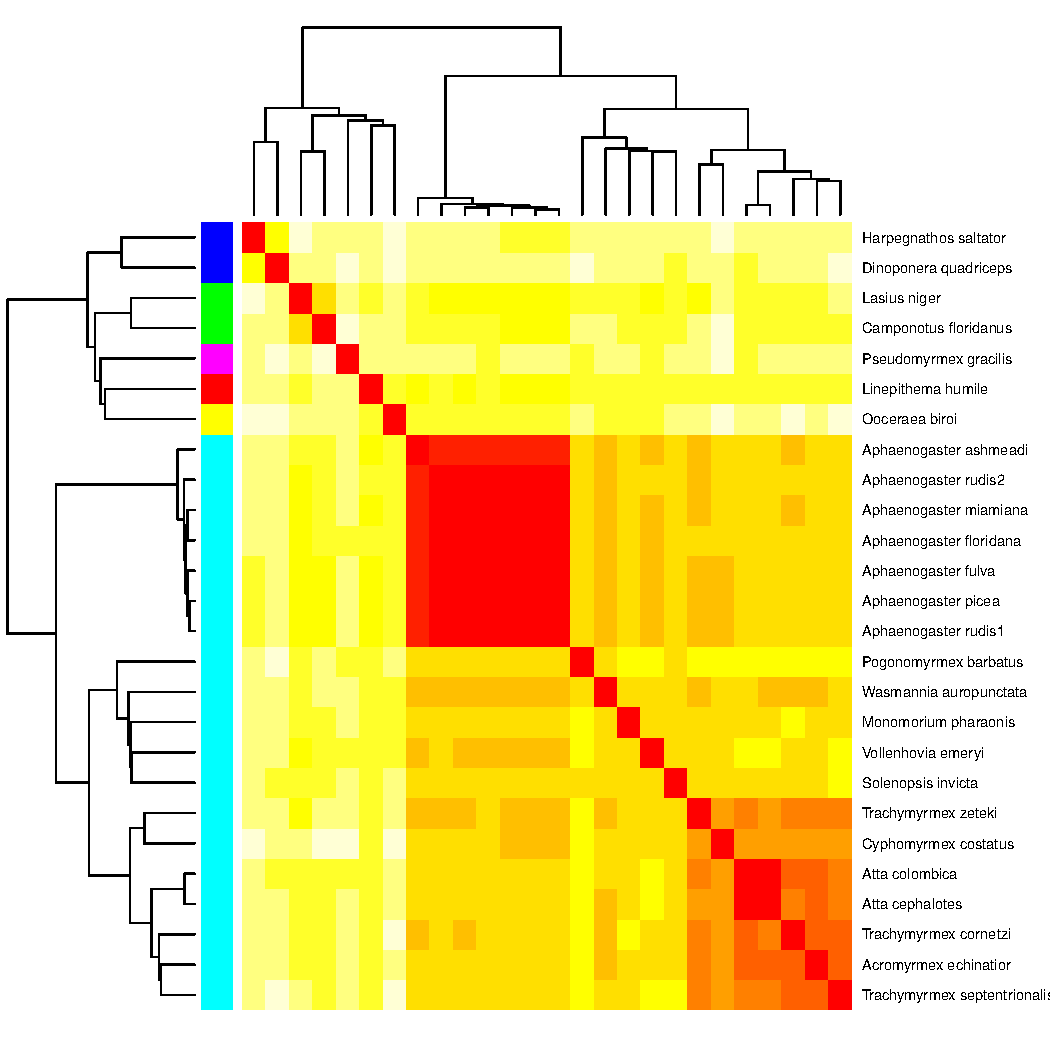
\includegraphics[width = 1\textwidth]{ncbi_heat.pdf}
\caption{Heatmap of the MASH genomic distances of the
  \textit{Aphaenogaster} species that we sampled together with other
  ant species in NCBIs. Heat colors shown in the central matrix range
  from high (white = 1) through moderate (orange = 0.5) to low (red =
  0) genomic distance; the diagonal is entirely red because it
  illustrates the distance of each sequence to itself. The cladograms
  on the left and top show hierarchical clustering of the
  genomes. Colors shown to the left of the matrix indicate ant
  subfamilies:  \emph{Ponerinae} (dark blue), \emph{Formicinae}
  (green), \emph{Pseudomyrmecinae} (pink), \emph{Dolichoderinae}
  (red), \emph{Dorylinae} (yellow), \emph{Myrmicinae} (light blue).}
\label{fig:all_heat}
\end{figure}


\subsection*{Biogeographic Patterns of Genomic Structure}

To examine these relationships, we conducted multivariate correlation
analyses (Mantel Tests) of interspecies whole-genome size similarity
using the Euclidean distance of whole-genome length (total base pairs)
and genomic similarity (MASH distance) with the Euclidean distances of
standardized climate variables. More specifically, we conducted
directional (H$_{\circ}$: Mantel r $\leq$ 0) partial mantel tests to control
for spatial autocorrelation by including geodesic distance as a term
\citep{Goslee2007}. Data for climate variables for each sampling
location from the WorldClim database (version 2.0) at a 2.5 arc minute
spatial resolution from the years 1970 to 2002 \citep{Fick2017}
(Table~\ref{tab:wc_var}).

\input{wc_vars}

Using a permutational multivariate analysis of variance (PerMANOVA)
procedure, we parsed the individual variables that were correlated
with both genome size and MASH similarity. PerMANOVA is a flexible
multivariate analog of ANOVA that permits the use of a wider set of
similarity metrics to be used for the response matrix
\citep{Anderson2001}, such as the MASH distance. We ran a total of
10,000 permutations of the original distance matrices for each
statistical permutation procedure. We chose a subset of all possible
climate variables available via WorldClim for this analysis. A visual
inspection of the sampled climate variable correlations indicated that
the primary climate variables, mean annual temperature (MAT), annual
minimum temperature, annual maximum temperature, annual precipitation
and summer precipitation, represented the majority of climate
variation (Fig~\ref{fig:clim_cor}). Based on this, we only included these
variables, along with latitude and longitude coordinates, as factors
in the PerMANOVAs.

\begin{figure}[ht]
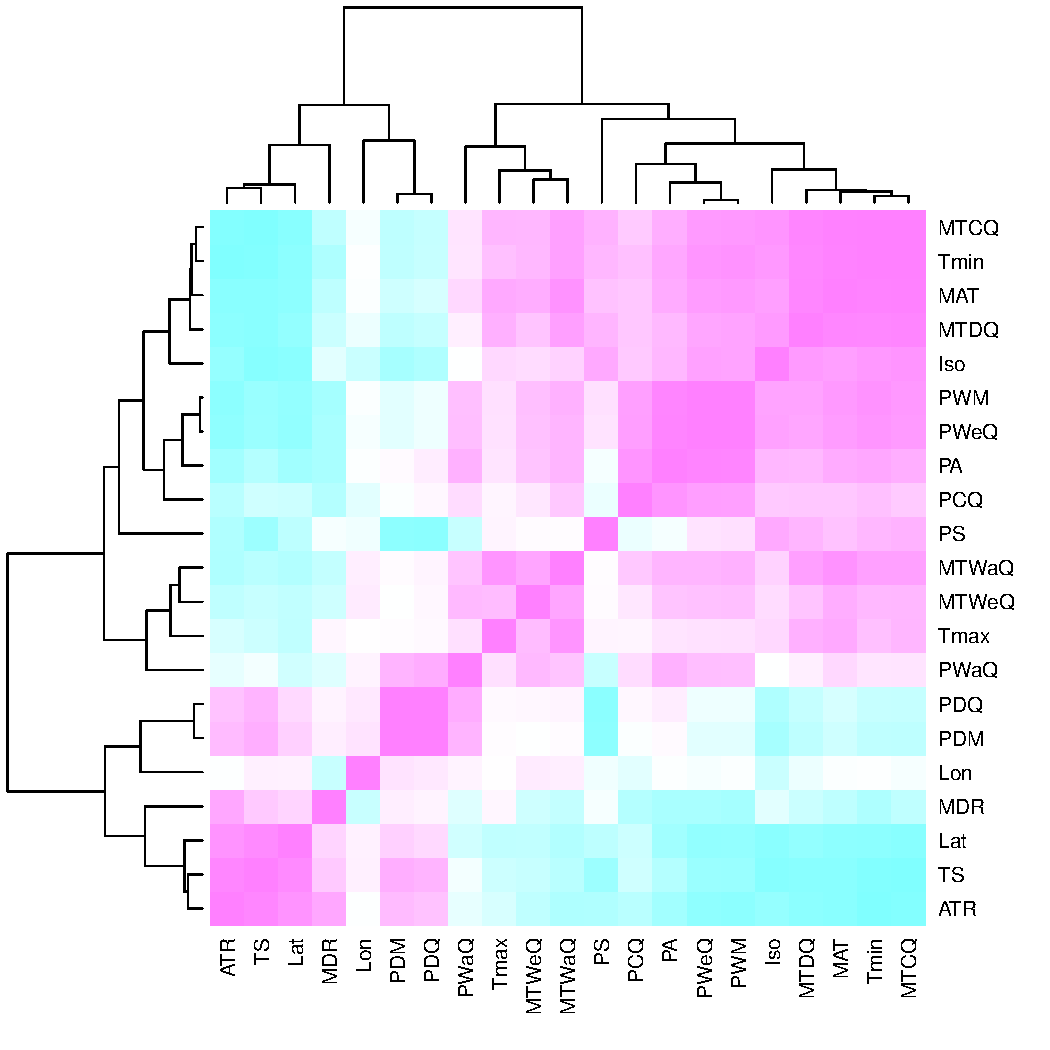
\includegraphics[width = 1\textwidth]{clim_cor.pdf}
\caption{Heatmap of Pearson correlations among climate
  variables. Cells in the heatmap are colored by the correlation
  between the two variables that intersect at that location ranging
  from blue = -1 to white = 0 to pink = 1. The variables are arrayed
  by hierarchical clustering of the correlations, as shown by the
  dendrograms on the top and left side.}
\label{fig:clim_cor}
\end{figure}

To visualize the patterns of genomic similarity and spatio-climate
variation, we used non-metric multidimensional scaling (NMDS)
ordination to the MASH genomic distances using 500 iterations to
produce a two-dimensional lowest stress solution for all genomes and
only the \textit{Aphaenogaster} genomes, respectively. The $R^2$ and
stress of the final solutions were 0.80 and 15\%. The geographic
(latitude and longitude) and WorldClim climate variables were then
correlated with both sets of MASH genomic distances (i.e. all and just
\textit{Aphaenogaster}) using a vector analyses \citep{Oksanen2016}.

We found significant global, biogeographic patterns of ant species
genomes. Across all whole-genome ant sequences (both the NCBI and the
newly sequenced \textit{Aphaenogaster} species), ants from
climatically similar locations tended to have similar genomes
(Fig~\ref{fig:wc_ord}). We also observed that collection location
climate similarity was significantly correlated with genome size
similarity (Mantel r = 0.19, \textit{p}-value = 0.021) and whole
genome similarity (MASH distance) (Mantel r = 0.3248169,
\textit{p}-value = 0.001).

\begin{figure}[ht]
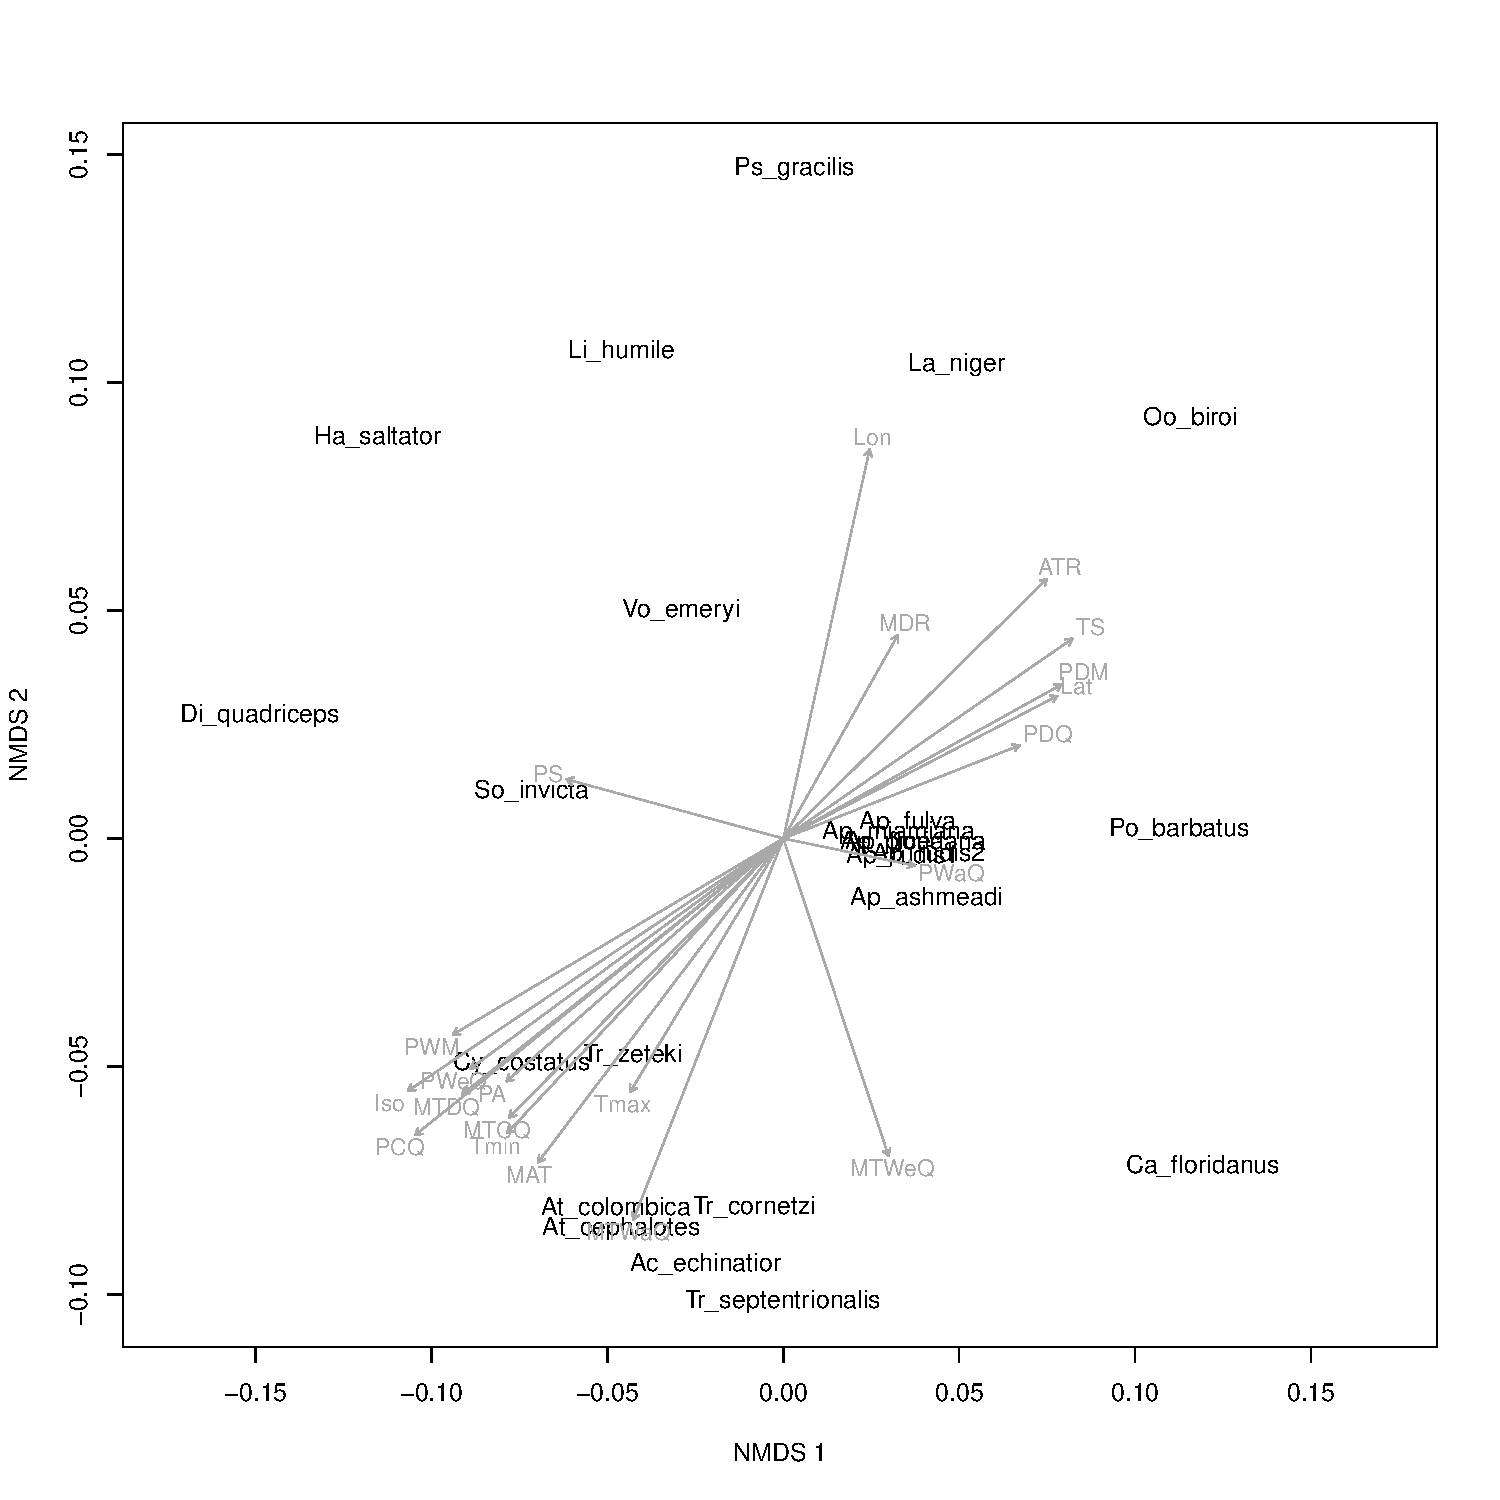
\includegraphics[width = 1\textwidth]{worldclim_ordination.pdf}
\caption{Plot an showing NMDS ordination of MASH genomic distance of
  all whole-genome ant sequences currently in NCBI and the newly
  sequenced \textit{Aphaenogaster} spp. from this study. Arrows
  overlaid on each plot show the correlation vectors (pointing in the
  direction of and scaled by the correlation) between the full set of
  climate variables from WorldClim at the sampling locations and the
  genomic distance of the samples.}
\label{fig:wc_ord}
\end{figure}

Both space and climate were important factors determining the size and
genomic similarity of the ant genomes. Longitude but not latitude was
a significant predictor of genome size
(Table~\ref{tab:perm_f}). Temperature of the coldest (Tmin) and
hottest (Tmax) month and total annual precipitation (PA), were all
significant predictors of genomic size similarity, but neither mean
annual temperature (MAT) nor summer precipitation (PS) were
significant predictors of genome size. Overall, Tmin was the strongest
predictor with an \textit{R}$^2$ of 0.23. Latitude and longitude were
both correlated with MASH genome distance; and all climate variables
examined were significant predictors of whole-genome similarity with
Tmin (\textit{R}$^2$ = 0.10) also being the strongest
predictor. Interestingly, when the newly sequenced
\textit{Aphaenogaster} genomes were excluded from the analysis,
climate was not correlated with genome size similarity (Mantel r =
0.13, \textit{p}-value = 0.190) and only annual precipitation (PA) was
a significant predictor of genome size similarity, and longitude and
mean annual temperature (MAT) were significant predictors of MASH
genomic similarity (Supplementary Materials Table 1).

\input{perm_f}

\subsection*{Data, Computation and Statistics}

The raw and assembled genome sequences are currently stored at Harvard
Forest (Petersham, MA, USA) and NCBI's genome database (Genome
Accessions NJRK00000000-NJRQ00000000 and BioSample Accessions
SAMN06892346-SAMN06892352). Genomic distance (MASH) computations were
run on the Odyssey cluster supported by the FAS Division of Science,
Research Computing Group at Harvard University. All analyses were
conducted in \textbf{R} \citep{RCoreTeam2017}. Analytical scripts for
the project are available online at the Harvard Forest Data Archive
(http://harvardforest.fas.harvard.edu/harvard-forest-data-archive). We
used the \textit{vegan} \citep{Oksanen2016} and \textit{ecodist}
\citep{Goslee2007} packages in R for the multivariate analyses.

\newpage
\clearpage

\section*{Discussion}

We have produced seven draft whole-genome sequences of six species of
ants in the genus \textit{Aphaenogaster}. These are the first
whole-genomes from a previously un-sequenced genus, adding to the
sequences of the diverse ``formicoid'' clade, which contains 90\% of
all extant ant species \citep{Ward2014}.  Our genomic sequences were
comparable in quality to other ant and insect genomes and the patterns
of genomic similarity were in line with expectations based on current
ant systematics. With the addition of these sequences, we observed
support for the hypotheses that genome size and similarity display
spatial patterns that relate to climate. Genomic patterns across
biogeographic gradients lend further weight to the importance of
considering the genetic basis of climate change responses.

Our results support the overarching perspective that climate has been
a force shaping the genetics of ant species. This is generally in-line
with previous observations of physiological and ecological responses
of ants to shifting temperatures \citep{Warren2013, Stanton-Geddes,
  Diamond2016, Nguyen2017, HelmsCahan2017, Diamond2017,
  Penick2017}. We observed a strong correlation between minimum
temperature and genome size and genomic similarity (MASH). Although
these results are correlative, they are also consistent with previous
research on the climatic determinants of ant distribution in North
America. For example, \citep{Warren2013} found that cold and not warm
temperatures limited shifts in the distributions of two
\textit{Aphaenogaster} species (\textit{A. picea} and
\textit{A. rudis}). With specific regard to genome size, the strong
correlation with minimum temperature points to altered genome size as
a potential indicator of a mechanism for adaptation to cold. The
findings of a recent, broad analysis of insect genome patterns
\citep{Alfsnes2017} has demonstrated support for climatic constraints
to genome size. One hypothesis being that cold temperatures could
select for smaller genomes \citep{Mousseau1997, Petrov2001,
  Alfsnes2017}.

It is important to consider that these biogeographic patterns could be
a function of other factors not examined in this study. We examined
the role of both space and climate; however, given the small sample
size of ant genomes we did not statistically control for
phylogeny. The genomic patterns we observed are likely to be a
function of both phylogeny and ecological variation, as previous
research has observed significant climate variation in insect genomes
even after controlling for phylogenetic relatedness
\citep{Alfsnes2017}. However, future work should disentangle the
partial correlations of phylogenetics and biogeographic variation in
ant genomes, once more sequences become available. In addition,
interactions of ants with other organisms are likely a strong factor
at play that could be a function of or interact with both space and
climate. For example, the distribution of the species \textit{Atta
  texana} is limited by the cold-tolerance of its fungal symbiont,
cultivars of the genus \textit{Attamyces} \citep{Mueller2011}. The
evolution of the ant-fungus relationship has lead to reductions in
some ant species ranges by cold temperatures. We observed patterns
corroborating this in our analysis in the correlation between
temperature variables and the clustering of similar genomes of ant
species from the tribe Attini (see Fig~\ref{fig:wc_ord}).

Further work investigating the variation in genomic content and
mapping of target coding regions from from previous experimental
physiological \citep{Nguyen2017}, biochemical \citep{HelmsCahan2017},
and transcriptomic \citep{Stanton-Geddes} work on
\textit{Aphaenogaster} and other ant species will inform predictions
of how these species and the ecosystems that they inhabit may respond
to ongoing climatic change. For example, determining the genomic
factors underlying the temperature response of ant assemblages to
climatic gradients \citep{Warren2013, Diamond2016, Diamond2017} could
provide useful insights into the response of these important organisms
to non-analog ecosystem states and idiosyncratic community responses
\citep{Bewick2014a}. Also, as species distribution models have been
significantly improved by the inclusion of genetic information
\citep{Ikeda2016}, an ecological genetics approach that couples ant
genomic and ecologically relevant data will likely provide a useful
window into the response of a range of terrestrial ecosystems to
climatic change.


\section*{Conclusion}

The addition of the \textit{Aphaenogaster} sequences have increased
the breadth of global ant genomic sampling. The total number of ant
sequences analyzed here is still a relatively small sample (n = 26) of
the estimated $>$16,000 ant species and subspecies (www.antweb.org,
accessed 16 April 2018). As the addition of the \textit{Aphaenogaster}
sequences had a marked impact on the statistical results of the
climate analysis, we expect that further sequencing work will continue
to shift our perspective of the ecological genomics of ants. Although
our analysis did include some statistical control of
spatial-autocorrelation, these results are still correlative and do
not eliminate other important factors that might covary with climate,
such as phylogeny. Additional analytical and experimental work will be
necessary to parse out a clearer understanding of the mechanisms
behind these patterns. New sequencing work has been initiated by The
Global Ant Genomics Alliance \citep{Boomsma2017}, which aims to
greatly increase the number of ant species sequenced from across the
world. These efforts will enhance our ability to resolve a clearer
picture of the future impacts of global climate change.

\section*{Acknowledgments}

Thank you to the team at the Broad Institute: particularly, James
Bochicchio, Sarah Young, Terrance Shay and Caroline Cusick. This work
was supported by a US National Science Foundation Dimensions of
Biodiversity grant (DEB 11-36646) to NJS, RRD, AME, NJG and SHC.

%% Our manuscript was written with \LaTeX~in \emph{Emacs} and
%% \emph{Overleaf} (\url{www.overleaf.com}).
%% We used the Mendeley citation manager.
%% So long and thanks for all the fish.


\newpage
\clearpage

\bibliography{apGenomes}

\clearpage

\section*{Supplementary Materials}

\setcounter{figure}{0}
\setcounter{table}{0}

\input{perm_f_napg} 

\end{document}
